\section{Bestimmung von $\kappa$ nach Rüchardt-Flammersfeld}
	
	\subsection{Methoden}
		
		Dieser Abschnitt beschäftigt sich mit dem Aufbau und der Funktionsweise des Teilversuches zur Bestimmung von $\kappa$ nach Rüchardt-Flammersfeld.
	
		\subsubsection{Aufbau}
		
			\begin{figure}[ht]
				\centering
				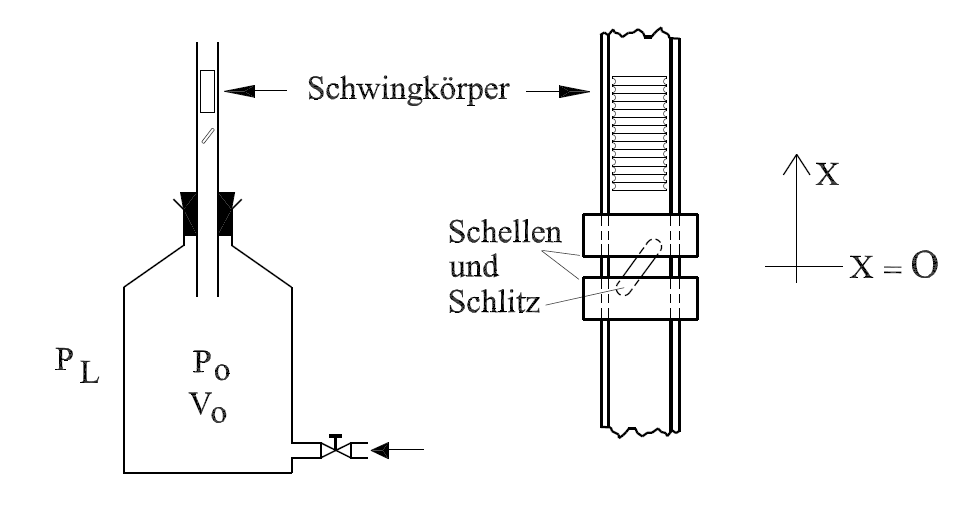
\includegraphics[width=0.8\textwidth]{bilder/aufbau_v1.png}
				\caption{.\cite{WWU}} %TODO caption
				\label{fig:AufbauV1}	
			\end{figure}
			Der Versuchsaufbau ist in Abbildung \ref{fig:AufbauV1} graphisch dargestellt.
			Zu erkennen ist, dass der Aufbau im Wesentlichem aus einer großen Flasche, in dessen langen Flaschenhals sich ein Schwingkörper befindet, besteht.
			Zusätzlich ist an dem Flaschenhals eine schlitzförmige Öffnung, dessen Größe sich durch die anliegenden Schellen beliebig anpassen lässt.
			Dieser Flaschenhals erweitert sich wie eine Röhre bis zum Flaschenboden, sodass der Schwingkörper nicht unten herausfallen kann, jedoch so, dass der Druck in dem Rohr unterhalb des Schlitzes dem Druck in der Flasche entspricht.		
			Bei diesem Druck handelt es sich um $P_0$, wie in der Abbildung verzeichnet. 
			Der Luftdruck definiert sich hier durch $P_L$.
			Unten, nahe dem Flaschenboden lässt sich ein Gas in diese einführen, sodass der Druck $P_0$ variiert werden kann.
			Die Flasche samt Rohr besitzt das Volumen $V_0$, wobei der Querschnitt des Flaschenhalses im Folgenden als $A$ bezeichnet wird. 
			Auch der Schwingkörper besitzt eine Querschnittsfläche von $A$, sodass das Gas in der Flasche nicht einfach entweichen kann. 
			
		\subsubsection{Funktionsweise}
			
			Ist der Druck $P_0$ nach dem Einführen eines Gases größer als der Luftdruck $P_L$, so beginnt der Schwingkörper aufwärts zu treiben.
			Steigt er über den Schlitz hinaus, entweicht Gas aus der Flasche und der Druck verringert sich wieder.
			Dies führt zu dem Fallen des Schwingkörpers.
			Bei konstanter Einführung eines Gases führt dies zu einer kontinuierlichen Erhöhung des Drucks $P_0$, welcher bei dem Erreichen des Schlitzes wieder abfällt und daraufhin erneut steigt.
			Aus dieser Bewegung stammt der Name des Schwingkörpers.
			Hierbei handelt es sich um eine ungedämpfte Druck- und Volumenschwingung des Gases.
			Dieser Vorgang verläuft adiabatisch, da die Änderungen von Druck und Volumen schnell genug erfolgen, dass ein Temperaturausgleich mit der Umgebung nicht stattfinden kann.
			Reibungsverluste werden über die konstante Zufuhr an Energie an den Schwingkörper durch eine schwache Gaszufuhr kompensiert.
			 
			Ist der Schwingkörper in seiner Gleichgewichtslage, so gilt:
			\begin{equation}
				P_0 = P_L + \frac{m\cdot g}{A},
			\end{equation} 
			wobei $m$ der Masse des Schwingkörpers ist und der Bruch den Druck beschreibt, den der Schwingkörper auf die Flasche (und deren Inhalt) auswirkt.
			
			Aus den Poissonschen Gleichungen für adiabatische Zustandsänderungen, $\Delta V = Ax$ mit $x$ als Position des Schwingkörpers lässt sich über das Aufstellen einer Bewegungsgleichung für einen linearen harmonischen Oszillator der Adiabatenexponent $\kappa$ bestimmen:
			\begin{equation} \label{eq:kappav1}
				\kappa = \frac{4\pi^2mV_0}{P_0A^2T^2},
			\end{equation}
			dabei ist $T$ die Zeit für eine Schwingungsdauer, welche aus der Gleichung für den harmonischen Oszillator stammt.
			
			Somit lässt sich der Adiabatenexponent $\kappa$ für verschiedene Gase bestimmen, indem konstant Gas zugeführt wird und die Schwingungsdauer $T$ gemessen wird. 
			
	\subsection{Durchführung}
		
		Zur Bestimmung des Adiabatenkoeffizienten $\kappa$ für die Gase/Gasverbindungen Luft, Argon und Kohlenstoffdioxid wurden die Schwingungsdauern $T$ für 100 Schwingungen pro Gas, bei Spaltbreiten von \SIrange{0,5}{3}{\milli\meter} in Abständen von \SI{0,5}{\milli\meter}, verzeichnet. % TODO Unsicherheiten
		Da die Schwingungen auch bei schwacher Gaszufuhr schnell verliefen, lag die Schwierigkeit an diesem Versuch daran, die Zeit bei der verwendeten Stoppuhr nach genau 100 Schwingungen zu stoppen.
		Der Gasstrom wurde so gewählt, dass die Schwingung symmetrisch zu dem Schlitz erfolgte.
		Nach jeder Messung wurden Rohr und Schwingkörper durch Putzen von störenden elektrischen Aufladungen befreit.
		
		Das Gewicht des Schwingkörpers wurde mit einer Waage auf $m = \SI{7,1}{\gram}$ bestimmt. % TODO Unsicherheit
		Der Luftdruck $P_L$ befand sich während des Versuches bei $P_L = \SI{1008,7}{\milli\bar}$. % TODO Unsicherheit
		Und für die Querschnittsfläche wurde über den Durchmesser von \SI{15,9}{\milli\meter} des Flaschenhalses eine Fläche von $A = \SI{}{\milli\meter^2}$ bestimmt. % TODO Wert A, Unsicherheit
		Das Volumen der Flasche war auf dieser angegeben: $V_\text{Flasche} = \SI{5450}{\centi\meter^3}$ und das des Rohres entspricht obigem $\Delta V$.
		$V_0$ ergibt sich aus der Summe der beiden Volumina.
		
	\subsection{Datenanalyse}
	
		Die Tabelle mit den aufgezeichneten Schwingungsdauern ist dem Laborbuch zu entnehmen.
		Da diese sich für verschiedene Größen des Schlitzes bei gleichem Gas jedoch nur minimal voneinander unterscheiden und keine Proportionalität zu erkennen ist (vgl. Abb. \ref{fig:T/d}), sind nur die Mittelewerte in Tabelle \ref{tab:Werte1} aufgeführt.
		\begin{figure}[ht]
			\centering
			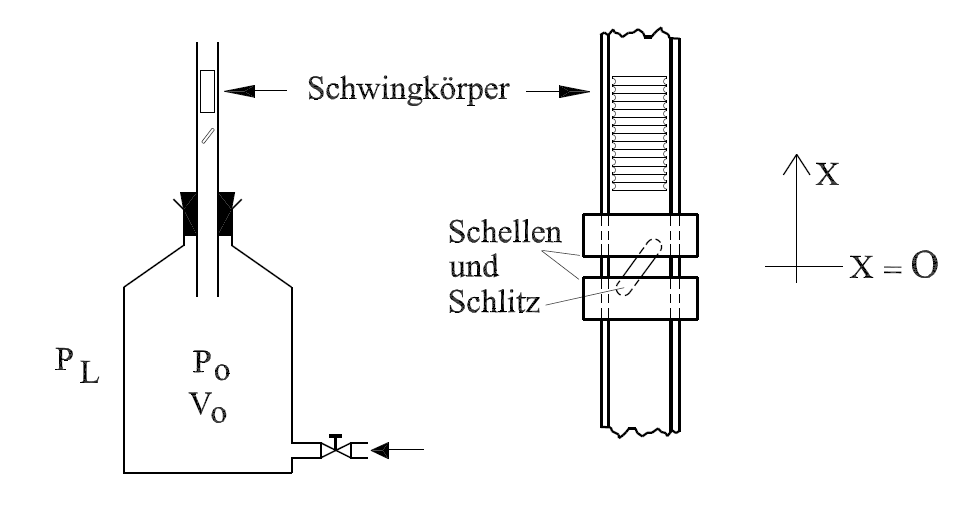
\includegraphics[width=0.8\textwidth]{bilder/aufbau_v1.png}
			\caption{.\cite{WWU}}
			\label{fig:T/d}	
		\end{figure}
		In dieser Tabelle sind zudem die aus Gleichung \ref{eq:kappav1} berechneten Adiabatenexponenten $\kappa$ für die jeweiligen Gase eingetragen.
		Da $\kappa$ gerade dem Verhältnis von spezifischer isobaren und spezifischer isochoren Wärmekapazität $c_p/c_V$ entspricht und diese in molarer Größe in direkter Verbindung mit dem Freiheitsgrad der Gase stehen folgt:
		\begin{equation} \label{eq:Freiheit}
		\kappa = \frac{c_p}{c_V} = \frac{f+2}{f}.
		\end{equation}
		Hierbei entspricht $f$ dem Freiheitsgrad des Gases.
		Aus Umformung lässt sich der Freiheitsgrad $f$ in Abhängigkeit von $\kappa$ bestimmen.
		Auch diese sind für die verschiedenen Gase in Tab. \ref{tab:Werte1} verzeichnet.
		\begin{table}
			\caption{In dieser Tabelle sind die Mittelwerte für die Schwingungsdauern $\bar{T}$ bei den verschiedenen verwendeten Gasen verzeichnet, sowie die zugehörigen Werte für die Adiabatenexponenten $\kappa$ und den daraus folgenden Freiheitsgraden}
			\label{tab:Werte1}
			\centering
			\begin{tabular}{c|c|c|c}					
				& Luft & Argon & Kohlenstoffdioxid\\
				\hline
				&&&\\ % Weil sonst der Mittelwertsbalken exakt auf der hline liegt
				$\bar{T}$ & & & \\ %TODO Werte
				$\kappa$ & & & \\ %TODO Werte
				$f$ & & & \\ %TODO Werte
			\end{tabular}
		\end{table} 
		
	\subsection{Diskussion}
	
		Nun stellt sich die Frage, ob die Ziele der Untersuchung erreicht wurden.
		Dazu wird zunächst betrachtet, ob die ermittelten Freiheitsgrade sinngemäß sind.
		Für das einatomige Argon gehen nur die Freiheitsgrade der Translation, also drei ein.
		Berechnet wurden % TODO Wert, Erklärung
		Bei Luft, welches im Wesentlichen aus den zweiatomigen Molekülen $N_2$ und $O_2$ besteht gehen auch zwei zusätzliche Freiheitsgrade der Rotation ein. 
		Da hier jedoch auch bis zu zwei weitere über Schwingung möglich wären, ist zu erwarten, dass der berechnete Wert zwischen fünf und sieben Freiheitsgrade besitzt.
		Dies ist % TODO Wert, Erklärung
		Für das dreiatomige Kohlenstoffdioxid verläuft die Betrachtung ähnlich, hier sind jedoch mehr Freiheitsgrade über Schwingungen möglich.
		Zu erwarten wären hier für das (nicht) gestreckte $CO_2$ fünf bis dreizehn / sechs bis zwölf Freiheitsgrade.
		Mit % TODO Wert, Erklärung
		Da die Ergebnisse in Abhängigkeit von $\kappa$ berechnet wurden, ist eine mögliche Fehlerquelle ein falsch bestimmter Adiabatenexponent.
		Für die verschiedenen Gase finden sich folgende Literaturwerte: % TODO Werte
		Verglichen mit den Berechneten, liegen Abweichungen von % TODO Werte, Erklärung
		Dies zeigt, dass die Ziele der Untersuchung % TODO (nicht) erreicht wurden
